\documentclass{article}sepackage{graphicx}egin{document}

\begin{figure}[ht]
  \centering
  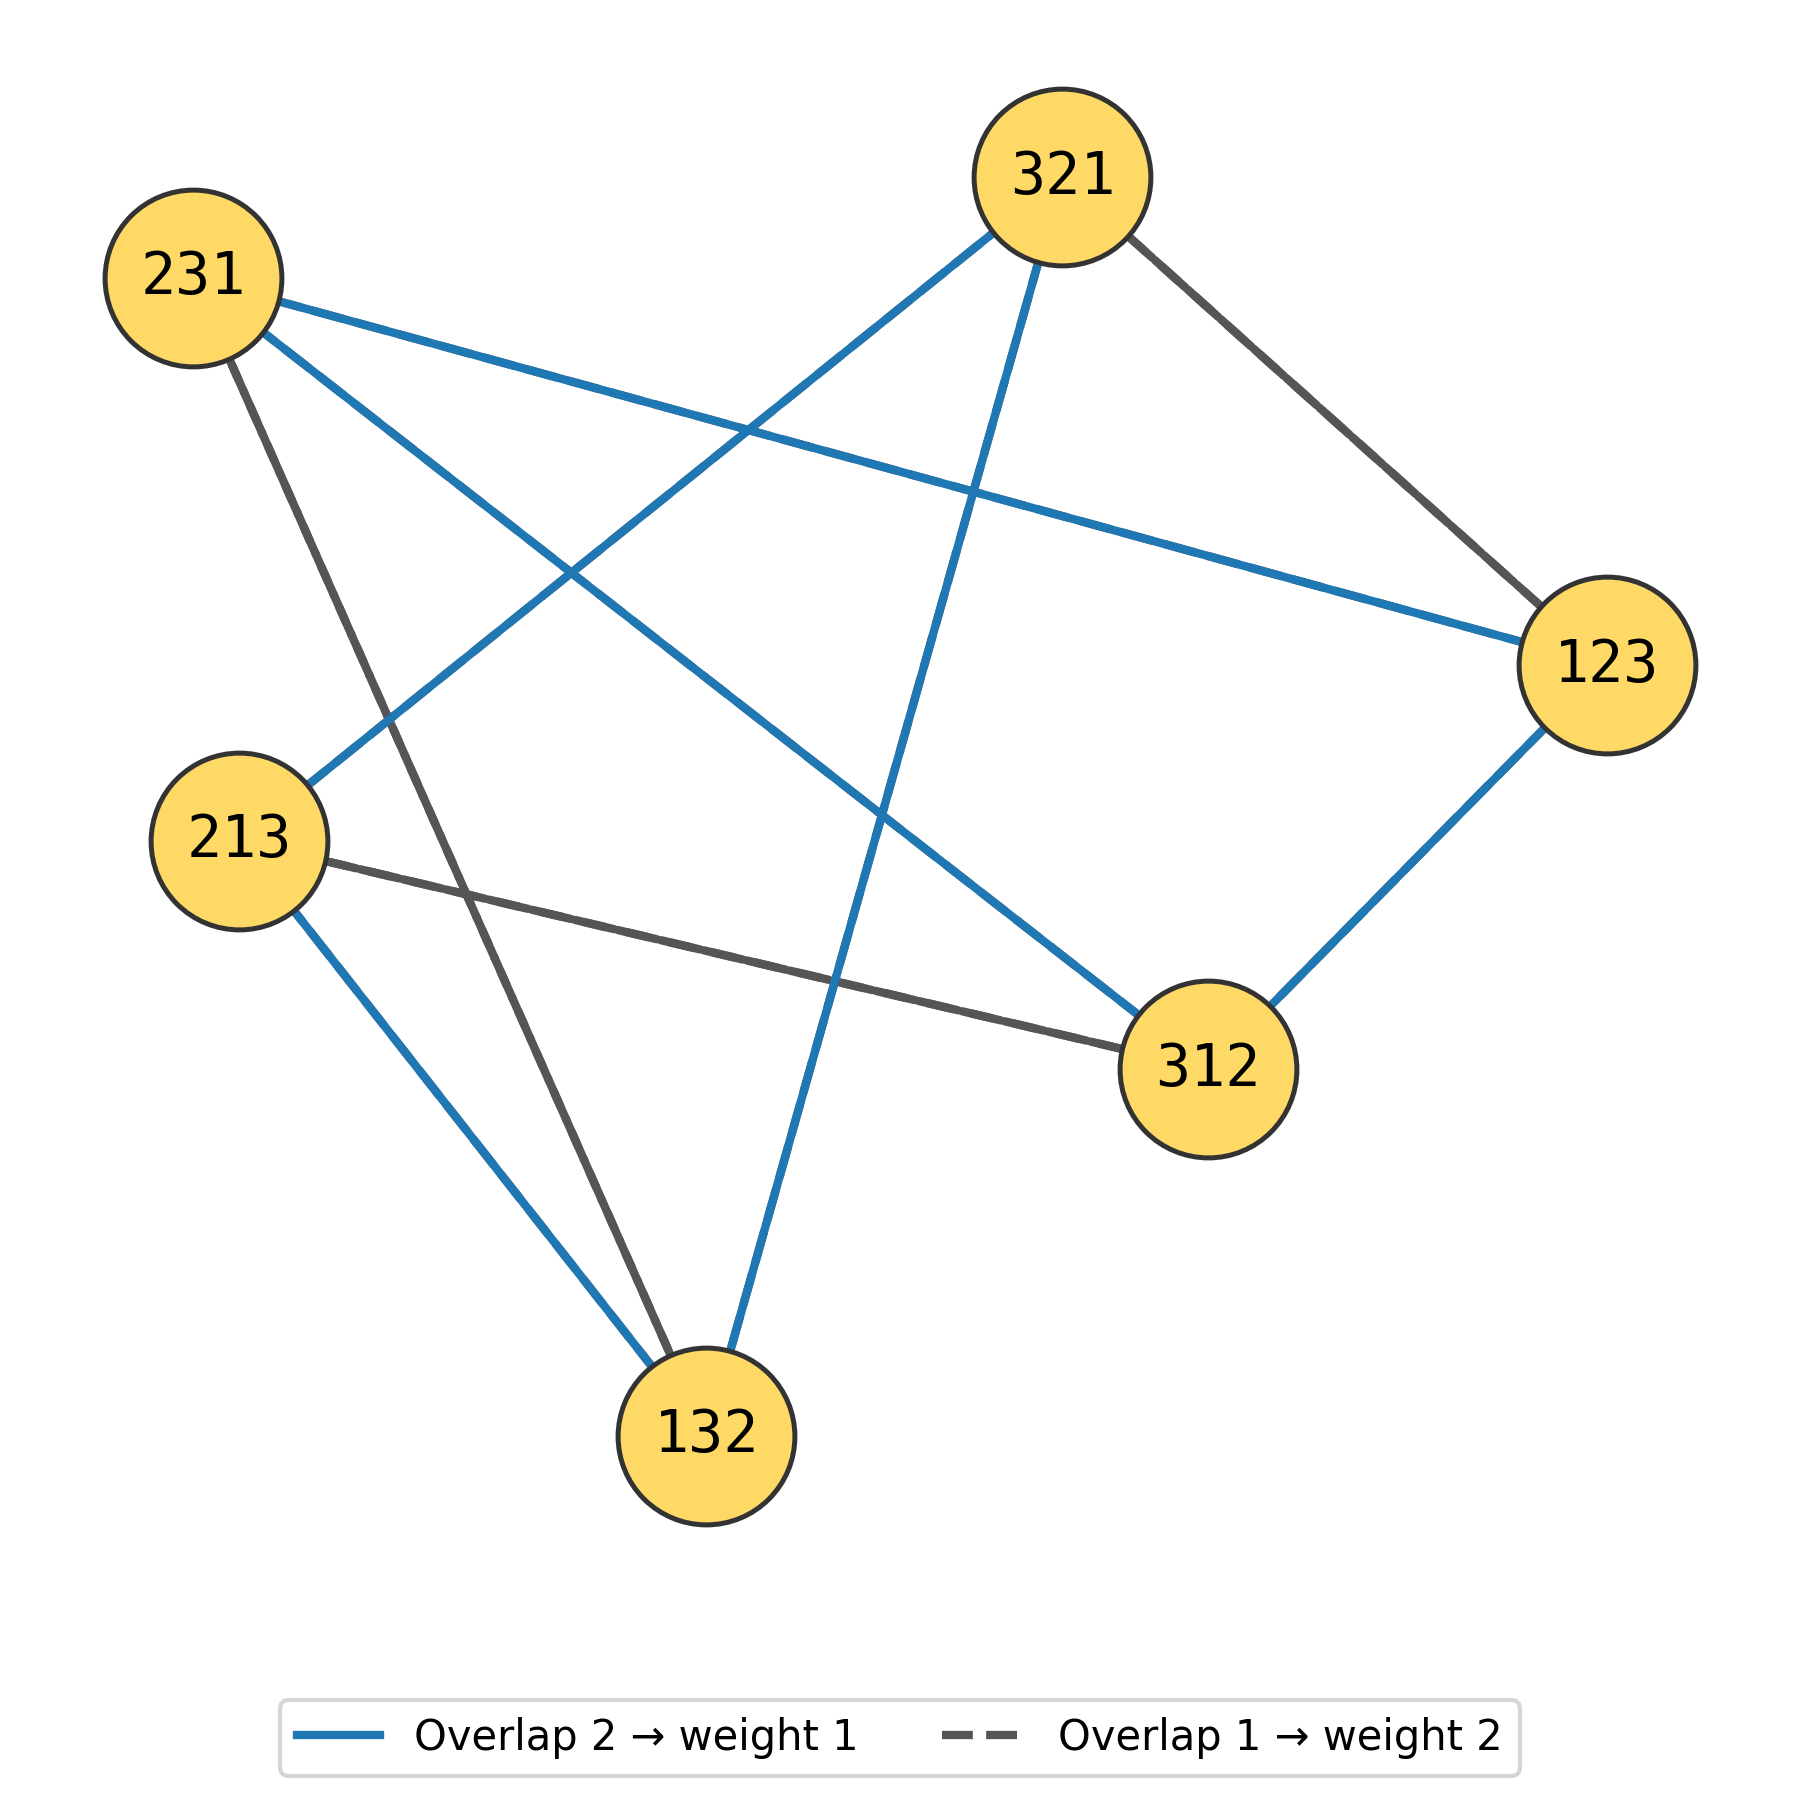
\includegraphics[width=0.7\textwidth]{39_SuperpermutationsBreakthrough/permutation_graph_n3_spring.png}
  \caption{Permutation graph for $n=3$. Each node is one of the six permutations of $\{1,2,3\}$. A directed edge $A\to B$ carries \emph{weight} $w=n-k$, where $k$ is the length of the longest suffix of $A$ matching a prefix of $B$; equivalently, $w$ is the number of extra symbols needed to append $B$ after $A$. Thus, an \emph{overlap} of two symbols ($k=2$) gives \emph{weight 1} (solid blue), and an \emph{overlap} of one symbol ($k=1$) gives \emph{weight 2} (dashed gray).}
  \label{fig:permgraph3}
\end{figure}

For small values of $n$, exact solutions have been found. Remarkably, for $n = 1$ through $n = 5$, the shortest superpermutations are known, and their lengths follow a simple closed-form pattern:
\[
nd{document}
